\documentclass[tikz,border=7pt]{standalone}
\usepackage{iftex}
\ifPDFTeX
  \PackageError{matrix-figure}{This figure requires XeTeX or Tectonic}{Compile with xelatex or tectonic.}
\fi
\usepackage{fontspec}
\usepackage{xeCJK}
\usepackage{amsmath}
\usepackage{unicode-math}
\usepackage{xcolor}
\usepackage{tikz}
\usetikzlibrary{arrows.meta,positioning}

\providecommand{\FigureUseLocalFonts}{0}
\ifnum\FigureUseLocalFonts=1
  \setmainfont{NotoSansCJKtc-Regular.otf}[Path=\FigureSansFontPath]
  \setsansfont{NotoSansCJKtc-Regular.otf}[Path=\FigureSansFontPath,BoldFont=NotoSansCJKtc-Bold.otf]
  \setCJKmainfont{NotoSansCJKtc-Regular.otf}[Path=\FigureSansFontPath]
  \setCJKsansfont{NotoSansCJKtc-Regular.otf}[Path=\FigureSansFontPath,BoldFont=NotoSansCJKtc-Bold.otf]
  \setmathfont{STIXTwoMath.otf}[Path=\FigureMathFontPath]
\else
  \setmainfont{Noto Sans CJK TC}
  \setsansfont{Noto Sans CJK TC}
  \setCJKmainfont{Noto Sans CJK TC}
  \setCJKsansfont{Noto Sans CJK TC}
  \setmathfont{STIX Two Math}
\fi

\definecolor{FigureInk}{HTML}{253142}
\definecolor{PanelFill}{gray}{0.96}
\definecolor{RowShade}{gray}{0.86}
\definecolor{ColumnShade}{gray}{0.74}
\definecolor{ResultShade}{gray}{0.58}
\definecolor{FocusShade}{gray}{0.68}
\definecolor{GuideShade}{gray}{0.80}

\newcommand{\MatrixCell}[2]{%
  \tikz[baseline=(value.base)]{\node[fill=#1,rounded corners=0.4pt,inner sep=2.2pt,
    minimum width=1.35em,minimum height=1.35em] (value) {$#2$};}%
}
\newcommand{\RowCell}[1]{\MatrixCell{RowShade}{#1}}
\newcommand{\ColumnCell}[1]{\MatrixCell{ColumnShade}{#1}}
\newcommand{\ResultCell}[1]{\MatrixCell{ResultShade}{#1}}
\newcommand{\FocusCell}[1]{\MatrixCell{FocusShade}{#1}}

\tikzset{
  figure/.style={font=\sffamily,text=FigureInk,>={Stealth[length=3.5mm,width=2.5mm]}},
  panel/.style={draw=FigureInk,line width=0.9pt,rounded corners=1.5mm,fill=PanelFill,align=center},
  flow/.style={-{Stealth},line width=1.05pt,draw=FigureInk},
}


\begin{document}
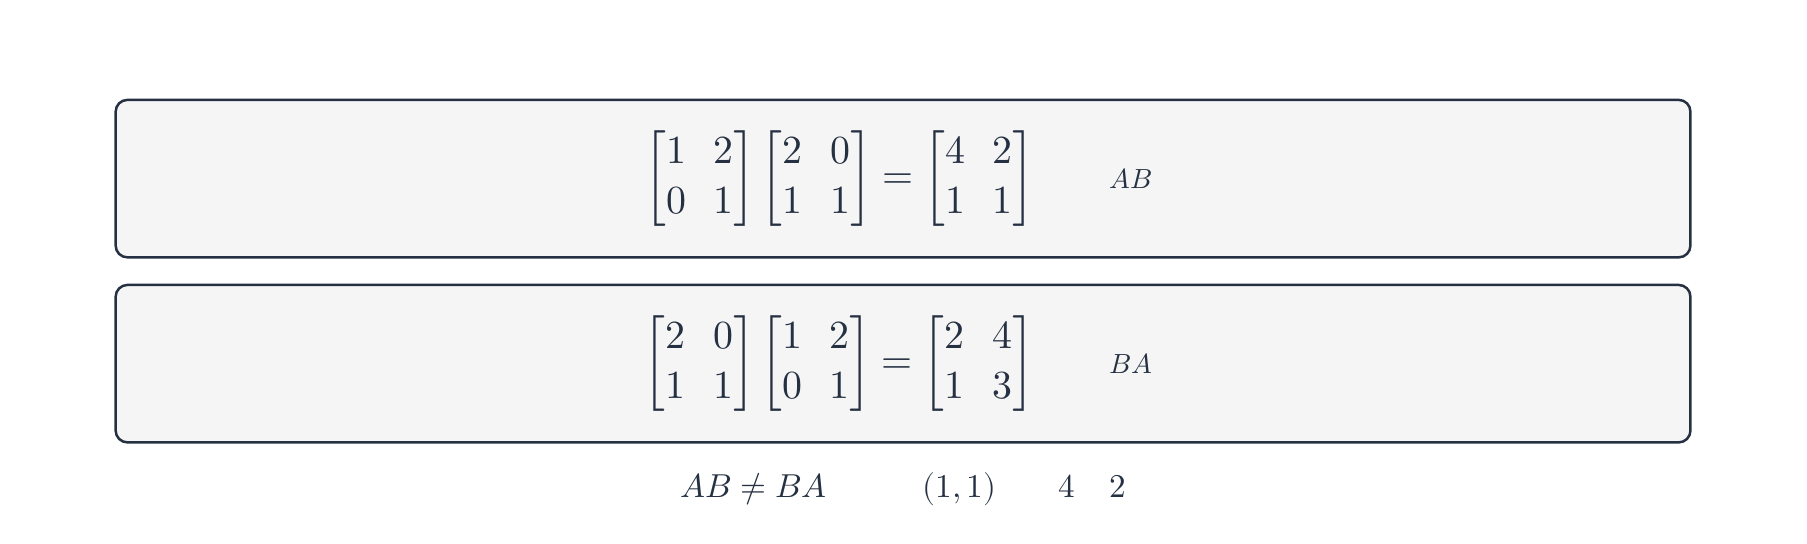
\begin{tikzpicture}[figure]
  \node[font=\bfseries\Large,align=center,text width=22cm] at (11,6.0)
    {交換矩陣的乘法順序會改變每一次列乘行的配對};

  \node[panel,minimum width=20.0cm,minimum height=2.0cm] at (11,4.2) {%
    \Large
    $\begin{bmatrix}1&2\\0&1\end{bmatrix}
     \begin{bmatrix}2&0\\1&1\end{bmatrix}
     =\begin{bmatrix}4&2\\1&1\end{bmatrix}$
    \hspace{8mm}\normalsize$AB$
  };

  \node[panel,minimum width=20.0cm,minimum height=2.0cm] at (11,1.85) {%
    \Large
    $\begin{bmatrix}2&0\\1&1\end{bmatrix}
     \begin{bmatrix}1&2\\0&1\end{bmatrix}
     =\begin{bmatrix}2&4\\1&3\end{bmatrix}$
    \hspace{8mm}\normalsize$BA$
  };

  \node[font=\bfseries\large] at (11,0.25)
    {$AB\ne BA$；例如兩個乘積的第 $(1,1)$ 元分別是 $4$ 與 $2$};
\end{tikzpicture}
\end{document}
